\documentclass[conference]{IEEEtran}
\usepackage[T1]{fontenc}
\usepackage{amsmath}
\usepackage{graphicx}
\usepackage{booktabs}
\usepackage{tabularx}
\usepackage{algorithm}
\usepackage{algpseudocode} 
\usepackage{hyperref}
\usepackage{enumitem}

% Title creation and placement.
\title{Proposal Document for Project I}
\author{
    \IEEEauthorblockN{Gianluca D'Altorio}
    \IEEEauthorblockA{Department of Computer Engineering Technology\\
    Vanier College}
}\date{\today}

\begin{document}
\maketitle

% Section 1: Problem Statement and User Need
\section{Problem Statement and User Need}
\label{sec:problem}

As people age, day-to-day tasks that were once routine become increasingly difficult, yet many older adults choose to live independently despite this.  An elderly person living alone who falls has no reliable way of summoning help, and caregivers or family members have no way of knowing something happened until it's too late.

This gap affects three primary groups directly: the elderly individual living alone, who bears the immediate risk of a fall, the caregiver or family member that is directly responsible for their well being, and the care facility who need to keep constant track of their patients.  Table~\ref{tab:needs} lists the possible needs of every stakeholder:

\begin{table}[!ht]
\centering
\caption{Provisional user needs, by stakeholder.}
\label{tab:needs}
\begin{tabularx}{\linewidth}{@{}l X@{}}
\toprule
ID & Need \\
\midrule
\multicolumn{2}{@{}l}{\textit{User (Wearer)}} \\
N1 & ``If I fall and can't get up, I need help to come without me having to do anything.'' \\
N2 & ``I want to be able to cancel an alert if I am fine before anyone is bothered.'' \\
N3 & ``I don't want to feel as though I am constantly being watched.'' \\
\addlinespace
\multicolumn{2}{@{}l}{\textit{Caregiver / Family}} \\
N4 & ``I need to be notified immediately if something happens.'' \\
N5 & ``I want to know if they are incapacitated after the fall.'' \\
N6 & ``I don't want to spend so much money on this device.'' \\
\addlinespace
\multicolumn{2}{@{}l}{\textit{Care Facility}} \\
N7 & ``I need alerts to be routed reliably so that response protocols are followed.'' \\
\addlinespace
\multicolumn{2}{@{}l}{\textit{Personal}} \\
N8 & ``The device firmware needs to be reproducible on new devices without editing the source.'' \\
\bottomrule
\end{tabularx}
\end{table}

Taken together, these needs point to one measurable target for the system as a whole, stated below as the project objective:\\

\textbf{Objective --} Prioritizing missed falls is the more serious failure mode: detect at least $95\%$ of real falls (miss rate $\leq 5\%$) and deliver a confirmed alert to the caregiver/family and care facility within 30 seconds, accepting a higher tolerance for false alarms ($\leq 10\%$) in exchange.

% Section 2: Scope and System Context
\section{Scope and System Context}
\label{sec:scope}

Meeting these needs requires deciding, upfront, what this system will and will not attempt in this term to ensure completion.  Table~\ref{tab:scope} lists what is built agianst the nearest capability deliberately left out, so that the boundary of the prototype is explicit rather than assumed. 

\begin{table}[!ht]
\centering
\caption{Scope of the proposed prototype.}
\label{tab:scope}
\begin{tabularx}{\linewidth}{@{}X X@{}}
\toprule
In Scope & Out of Scope \\
\midrule
Wrist IMU-based fall detection (watch). & Detecting other health events (seizures, cardiac events, etc). \\
\addlinespace
Waist IMU and barometric sensing (custom PCB). & Additional sensors (impact, heart rate, microphone, etc). \\
\addlinespace
Low-fidelity prototype development (breadboard/protoboard). & Custom PCB fabrication, enclosure, manufacturing/cost analysis. \\
\bottomrule
\end{tabularx}
\end{table}

Figure~\ref{fig:context} shows the system as a single boundary containing the fall-detection system, with no internal structure drawn at this stage.  The wearer's motion crosses into the system, and a confirmed alert crosses out to a computer running an MQTT broker, which pushes the notification to a caregiver-facing dashboard.  Two further stakeholders, the caregiver/family member and the care facility, sit downstream of the dashboard and are each reached independently.

% Figure 1.
\begin{figure}[!ht]
    \centering
    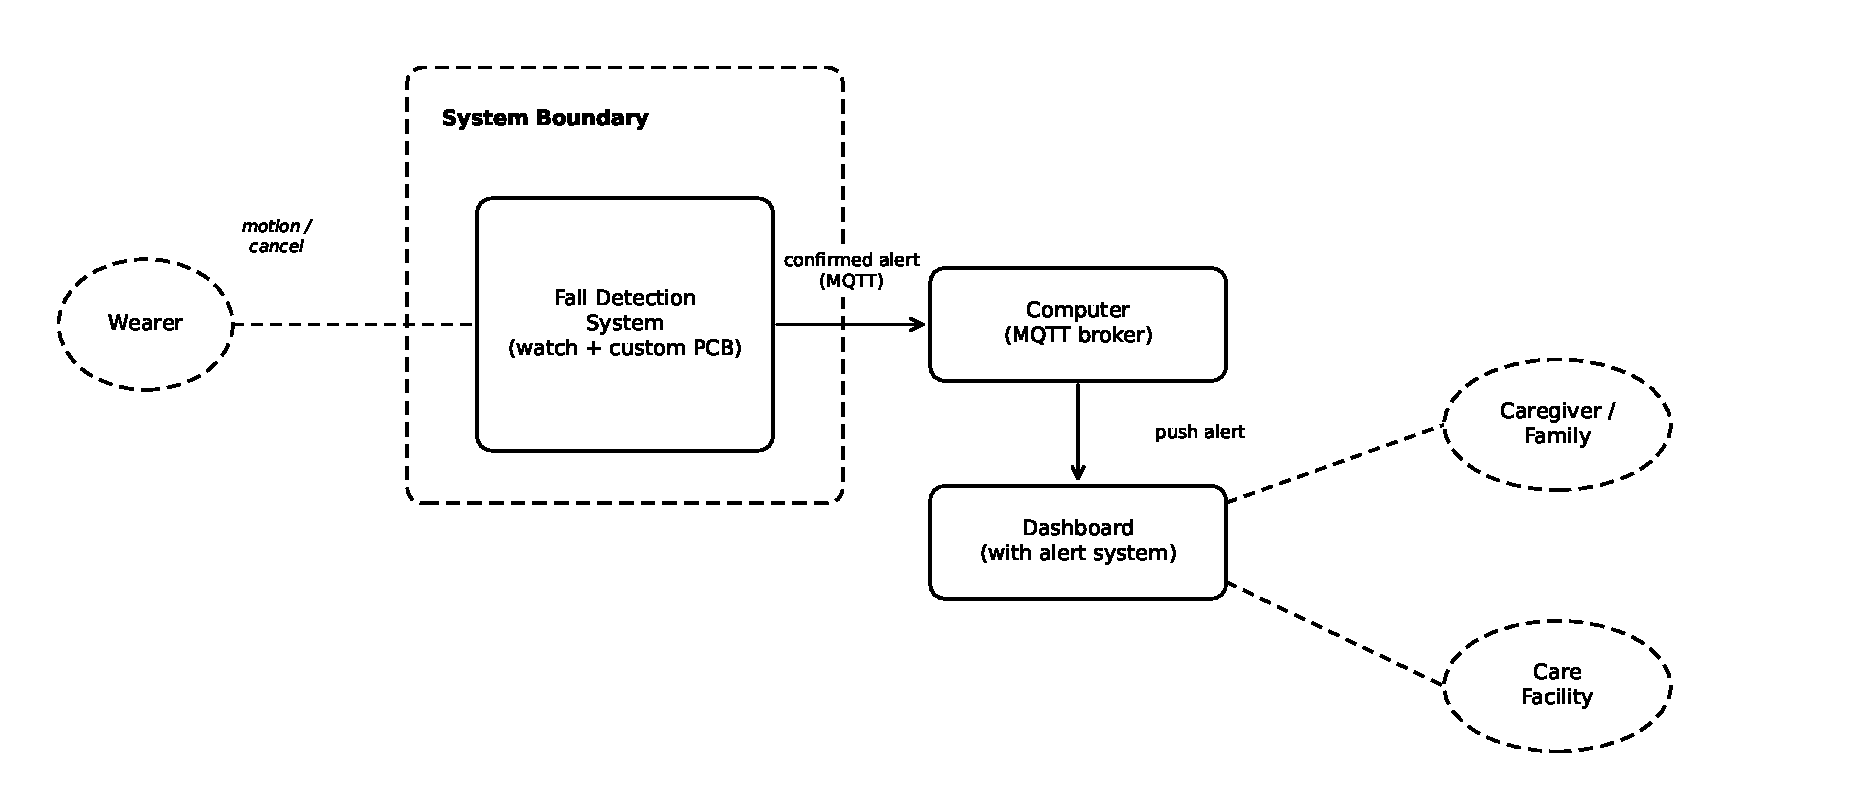
\includegraphics[width=\columnwidth]{figures/generated/context_diagram.pdf}
    \caption{System context diagram.  The wearer's motion enters the system for processing, 
    and is then moved downstream to the remaining stakeholders.}
    \label{fig:context}
\end{figure}

Two stakeholders behind this diagram want different things from the same design decision.  The wearer's success criterion is retaining the ability to cancel a false trigger before anyone is bothered (N2); the caregiver's is being notified the instant a fall occurs, with no delay standing between a real emergency and their response (N4).  These two criteria collide directly: any nonzero cancel window granted to the wearer is time subtracted from how quickly the caregiver can be alerted to a genuine fall.  No single window length fully satisfies both, and resolving this trade-off, choosing and defending a specific cancel-window duration, is one of the provisional requirements addressed in Section~\ref{sec:requirements}

% Section 3: Platform and Custom Hardware
\section{Platform and Custom Hardware}
\label{sec:platform}

The watch imposes several fixed limits on this design.  Table~\ref{tab:platform} lists only the specifications this project actually touches, each tagged with its source and marked as a constraint.

\begin{table}[!ht]
\centering
\small
\caption{Platform limits touched by this project, tagged as constraints.}
\label{tab:platform}
\begin{tabularx}{\linewidth}{
  @{}>{\raggedright\arraybackslash}p{0.06\linewidth}
    >{\raggedright\arraybackslash}p{0.28\linewidth}
    >{\raggedright\arraybackslash}p{0.15\linewidth}
    >{\raggedright\arraybackslash}X@{}}
\toprule
ID & Limit & Source & Rationale \\
\midrule
C1 & 6-axis IMU (wrist) & Vendor wiki & Fixed sensing hardware the wrist-side fall classifier runs on. \\
\addlinespace
C2 & Bluetooth 5 (LE) & Vendor wiki & Fixed radio the watch to PCB validation link and alert-to-broker path depend on. \\
\addlinespace
C3 & 2.4 GHz Wi-Fi (802.11 b/g/n) & Datasheet & Fixed radio for the MQTT alert path to the computer. \\
\addlinespace
C4 & ESP32-S3R8, dual core, up to 240\,MHz & Vendor wiki & Fixed processing budget the on-device fall classifier must run within, in real time. \\
\bottomrule
\end{tabularx}
\end{table}

The custom hardware is a waist-worn protoboard carrying its own microcontroller with an integrated BLE radio, a 6-axis IMU, and a barometric pressure sensor powered independently of the watch.  Since it is worn separately rather than physically attached, it cannot reach the watch's I2C, UART, or USB expansion pads; instead, the two devices exchange fall-event and validation data wirelessly over Bluetooth Low Energy.  This link is the subject of REQ-FD-07 in Section~\ref{sec:requirements}, which bounds how quickly a candidate fall event must reach the watch for validation.

% Section 4: Provisional Requirements
\section{Provisional Requirements}
\label{sec:requirements}

Table~\ref{tab:requirements} lists eight provisional requirements derived from the needs in Section~\ref{sec:problem}, covering all five requirement classes. Each is marked provisional, since none has yet been tested; Section~\ref{sec:uncertainties} treats the numeric bounds still resting on unvalidated assumptions as uncertainties to be resolved before Stage~1.

\textbf{Trial counts.} Rate-based criteria (REQ-FD-03) use $N=20$ trials per category, since at this count each trial corresponds to a $5\%$ increment, matching the resolution of the stated miss-rate threshold. Binary pass/fail requirements (REQ-FD-01, REQ-FD-04, REQ-FD-05, REQ-FD-07, REQ-FD-08) use $N=10$ repetitions, enough to catch an intermittent failure (a dropped connection, a timing race) without requiring the statistical power a rate claim needs.

\textbf{A note on these thresholds.} The numeric bounds in REQ-FD-02, REQ-FD-03, REQ-FD-05, REQ-FD-06, and REQ-FD-07 are each derived from a stated assumption or an existing figure in this table, not asserted without reasoning, but none has yet been validated by measurement. REQ-FD-06's cost cap, in particular, rests on a rough component estimate rather than an actual quotation. Any revision made after PoC testing or further research will be recorded as a new dated logbook entry.

% Section 5: Uncertainties and the PoC Plan
\section{Uncertainties and the PoC Plan}
\label{sec:uncertainties}

Three uncertainties are ranked below by how much of the design would collapse if the underlying assumption proved false, per the course guide's own rule for ranking.  Each is written as a register entry; the single PoC plan attacks the highest-ranked uncertainty first.

\textbf{PoC Plan.} The highest-ranked uncertainty, R1, is attacked first, since it would most undermine the design if wrong. \emph{Question:} what false-alarm and miss rates occur in the system when combining independent fall signals from two separate sensors, and does a confirmed fall reach its destination in time, even over a poor connection? \emph{Measure:} (a) false-alarm and miss rates on held-out data from a labeled set of scripted falls and confusable activities (sitting heavily, lying down, stairs), held out by session and, where possible, by person; (b) detection-to-dashboard delivery time and success rate at strong and weak link strength, and the system's behavior when the link is lost. \emph{Pass criterion, fixed in advance:} the miss rate is at most 5\%, the false-alarm rate is below 10\% (REQ-FD-03), and every confirmed fall is delivered within 30\,s (REQ-FD-02) in all link conditions tested.

% Source file for Table 4.
% Required in order for the reference in "proposal.tex" to work properly.

\begin{table}[!ht]
\centering
\caption{Provisional requirements (all unverified; marked provisional).}
\label{tab:requirements}
\scriptsize
\renewcommand{\arraystretch}{0.85}
\setlength{\tabcolsep}{3pt}
\begin{tabularx}{\linewidth}{@{}
  >{\raggedright\arraybackslash}p{0.06\linewidth}
  >{\raggedright\arraybackslash}p{0.065\linewidth}
  >{\raggedright\arraybackslash}p{0.21\linewidth}
  >{\raggedright\arraybackslash}p{0.265\linewidth}
  >{\raggedright\arraybackslash}p{0.22\linewidth}
  >{\raggedright\arraybackslash}p{0.055\linewidth}@{}}
\toprule
ID & Class & Statement & Rationale & Method/Acceptance & Need \\
\midrule
REQ-FD-01 & Func. & Initiate alert on fall, no wearer action. & A fall can incapacitate the wearer instantly, help can't depend on their own input (N1). & Demo: alert on sim.\ fall, $N{=}10$. & N1 \\
REQ-FD-02 & Perf. & Deliver alert within 25\,s, including over a degraded link. & 25\,s = 15\,s cancel (REQ-05) + 10\,s margin; board$\to$watch sub-link budgeted 200\,ms ($<$1\% of total). & Test: detect-to-receipt $\Delta$, $N{=}20$, strong/weak link; board$\to$watch $\Delta$ separately. & N1,4,7 \\
REQ-FD-03 & Perf. & Miss rate $\leq 5\%$ across tested activities. & Missed falls are worse than false alarms, per objective; 5\% matches 95\% target. & Test: false negatives / fall trials, $N{=}20$ held-out. & N1,4 \\
REQ-FD-04 & Perf. & False-alarm rate $< 10\%$ across tested activities. & Loosened to avoid suppressing true detections (REQ-03); still bounds nuisance interruptions to roughly 1 in 10 activities. & Test: false pos.\ / non-fall trials, $N{=}20$ held-out. & N2,3 \\
REQ-FD-05 & Interf. & Cancel pending alert via button within 15\,s. & Fixed independently as the wearer-reaction window; the remaining 10\,s of the 25\,s budget (REQ-02) covers transmission. Resolves wearer/caregiver collision (Sec.~\ref{sec:scope}). & Test: trigger-to-press $\Delta$, $N{=}10$; cancels only within window. & N2 \\
REQ-FD-06 & Func. & Escalate severity after 60\,s no post-fall motion. & $\sim$3$\times$ typical 10--20\,s stumble-recovery time. & Test: $\Delta$ to escalation, $N{=}10$; fires/withholds correctly. & N5 \\
REQ-FD-07 & Constr. & Added hardware cost $\leq$ \$45. & Caregiver cost concern (N6); rough BOM (MCU+BLE, IMU, barometer, battery, passives). & Inspect: receipts $\leq$ cap. & N6 \\
REQ-FD-08 & Build. & Firmware builds/flashes from clean checkout, one command, no edits. & Reproducibility (N8); commonly forgotten class. & Demo: build succeeds on 2nd machine. & N8 \\
\bottomrule
\end{tabularx}
\end{table}
\begin{table*}[!ht]
\centering
\footnotesize
\renewcommand{\arraystretch}{0.95}
\setlength{\tabcolsep}{3pt}
\caption{Ranked uncertainty register.}
\label{tab:uncertainties}
\begin{tabularx}{\linewidth}{@{}
  >{\raggedright\arraybackslash}p{0.025\linewidth}
  >{\raggedright\arraybackslash}p{0.19\linewidth}
  >{\raggedright\arraybackslash}p{0.155\linewidth}
  >{\raggedright\arraybackslash}p{0.155\linewidth}
  >{\raggedright\arraybackslash}p{0.045\linewidth}
  >{\raggedright\arraybackslash}p{0.17\linewidth}
  >{\raggedright\arraybackslash}p{0.17\linewidth}@{}}
\toprule
ID & Statement & Assumption & Consequence & Prob. & Evidence required & Mitigation \\
\midrule
R1 & The system may not meet the miss-rate and false-alarm targets together on data from people and sessions it was not tuned on. & Decision thresholds tuned on development sessions carry over to new wearers and sessions. & Objective missed: falls go undetected, or the wearer is bothered enough to stop wearing the device. & Unk. & False-alarm and miss rates measured on held-out sessions and at least one additional person, against the pass criterion. & If the PoC fails, retune the rule for combining the two signals or widen the training set. \\
R2 & 60\,s of post-fall inactivity may not reliably separate genuine incapacitation from a wearer resting deliberately. & Absence of motion for 60\,s after a confirmed fall is a meaningful proxy for incapacitation. & REQ-FD-05 could falsely escalate harmless events or fail to escalate a real emergency. & Unk. & Scripted trials of ``fall then rest'' vs.\ ``fall then recover,'' checked against escalation firing correctly. & Combine inactivity with a second signal, or retune the window based on measured separation. \\
R3 & BLE round-trip latency, worn on a moving body, may exceed the 200\,ms sub-budget assumed in REQ-FD-07. & Bench-measured BLE latency is representative of latency with both devices worn and the body in motion. & Total delivery time could exceed the 30\,s target (REQ-FD-02), or the cancel/detection time split would need revision. & Unk. & Timestamp-delta measurement with both devices worn during normal movement, not bench-only. & Re-split the 15\,s/30\,s budget, or tune BLE connection parameters to cut latency. \\
\bottomrule
\end{tabularx}
\end{table*}

% Section 6: Assumptions and the Logbook
\section{Assumptions and the Logbook}
\label{sec:assumptions}

\textbf{Assumptions.} This design rests on several claims taken as true but not
yet tested:

\begin{itemize}[leftmargin=*]
\item Falls performed by healthy volunteers under scripted, controlled conditions are assumed to produce IMU and barometric signatures representative of an actual elderly fall.
\item Bluetooth Low Energy connectivity between a wrist-worn watch and a waist-worn custom PCB is assumed to remain reliable at typical in-home separation distances between the two devices.
\item The watch's processing budget (C4) is assumed sufficient to run the on-device fall classifier and corroboration logic within the real-time constraints implied by REQ-FD-07's 200\,ms target.
\end{itemize}

\textbf{AI-Assisted Steps.} An AI assistant was used throughout drafting to help interrogate needs into measurable requirements, classify requirements by type, check scope and needs for internal consistency, and review wording against the course guide's own rules (e.g., the Test-versus-Demonstration distinction, and the requirement that every requirement trace to a recorded need). Every AI-suggested number, rationale, and requirement statement was reviewed by the author and checked against the guide's examples before inclusion; the honest, unvalidated status of REQ-FD-02, REQ-FD-03, REQ-FD-05, and REQ-FD-06's numeric bounds (Section~4) reflects that review, rather than a figure accepted uncritically.

\end{document}